\documentclass[../../thesis.tex]{subfiles}

\begin{document}

\TODO{Introduce the section, what we think and the philosophy of presenting material in such a way.}

\section{Neural Network}

Ref is \cite{deeplearningbook} chapter 6. ISLRv2 chapter 10

\textit{Feedforward neural network}, \textit{artificial neural network}, \textit{multilayer perceptron} or simply \textit{neural network} is a fundemental model in machine learning, and more specifically in \textit{deep learning}. \TODO{History}

A neural network takes in a vector of $x \in \mathbb{R}^n$ variables and builds a nonlinear function $f(x)$ to predict the response $y\in \mathbb{R}^m$. In particular a neural network maps an input vector $x$ to an output vector $y$ through a series of non-linear functions of linear combinations of the input. This particular structure, presented in figure [fig of nn here] is what distinguishes neural networks from other nonlinear prediction models. The variables $x = [x_1,...,x_n]$ constitutes the units of \textit{input layer}. The intermediate layers are called the \textit{hidden layers}, and the final mapping to $y$ is called the \textit{output layer}.

A neural network is parameterized by a set of \textit{weight} matrices $W_i$ and \textit{bias} vectors $b_i$, together with a specified non-linear \textit{activation function} $\sigma$. Written out a $K$ layered neural network is given by 
\[ 
f(x) = f_o \circ f_K \circ \ldots \circ f_1(x),
\]
where 
$$f_i = \sigma(W_ix+b_i), \quad i \in \{1,...,K\},$$ 
and $f_o$ is the output layer whos form is application dependent. It is worth mentioning that $\sigma$ is applied pointwise.

Two of the most commonly used activation functions are $\text{Sigmoid}(x) = \tfrac{1}{1+\exp(-x)}$ and $\text{ReLU}(x) = \max(0,x)$.  

\TODO{Importance of activation functions. The role of ReLU in the development of modern ML}


\TODO{Sneak in something about universal approximation theorem}


\section{Convolutional Neural Network}



\section{Residual Neural Network}


\section{Representation Learning}

\TODO{Sneak in something about Gödel and Turing in terms of representation. There are many philosophical aspects of this}

\subsection{What is representation learning?}
Representation learning is a term not too easily defined, one reason being the abstraction level. It relates closely to \textit{representation} of information, and representation of information can be many things. Lets begin by walking through a familiar and illustrative example. Consider the base $10$ integer $4$, or your favourite number. The number can equivalently (in terms of information content) be expressed, that is represented, in any other base. The particular base we choose depends on our intention with the number. If we want to work with digital electronics, a binary representation ($10$) is very useful, as transistors has two states. When humans do arithmetic, base $10$ representations of the integers are very natural, as we have $10$ fingers. A particular representation of information can make a task easier or harder.
\\ The information content is unchanged by a change of representation between $4$ in base $10$, $10$ when written in base $2$ or \RN{4} when written in roman numerals. What is changed is the challenges or easiness or difficulty of certain information processing tasks. Representation learning is then the process of learning a certain representation of information. 

\subsection{What is a good representation?}

For any representations extracted of a non-invertible function, a downstream task can always be designed (in principle) to based on the lost information, hence achieve arbitrarily bad performance. The concept of universally good representations is therefore ill-defined. There is no free lunch in representation learning either. One must specify a set of predefined downstream tasks, and evaluate according to those. The goodness of a representation is determined by how easy it makes a subsequent task.

\subsection{Why do we care about representation learning?}

Representation learning is particularly interesting because it provides one way to perform unsupervised and semi-supervised learning. It promises to unlock deep learning for unlabeled datasets. Furthermore it is known that the performance of machine learning methods is heavily dependent on the choice of data representations. Therefore much of actual efforts in deploying machine learning algorithms revolves around constructing good data pipelines and data transformations that results in representations suited for the ML algorithm. Being able to automate such processes, i.e automatic feature engineering, would solve massive problems and ease the use of ML considerably. 

\TODO{Talk about the trend of pre-traied models, language representations, tokenization, GPT etc}

\section{Regularization}

What it is and why it is needed. Leaky relu. Other techniques.

\section{Transformers}

When was it introduced, and by whom?
What lead up to its creation?
Why and where is it now widely used? 


Wiki: A deep learning architecture based on the multi-headed attention mechanism proposed in the 2017 paper "Attention is all you need".

One fo the main novelties of the architecture is not relying on recurrence, and instead solely using the attention mechanism to capture dependencies between input and output. As recurrent models are, in computational aspects, inherently sequential, there are major challanges when training as context windows, and sequence lengths become longer. 



\subsection{The attention mechanism}

\begin{figure}[h]
    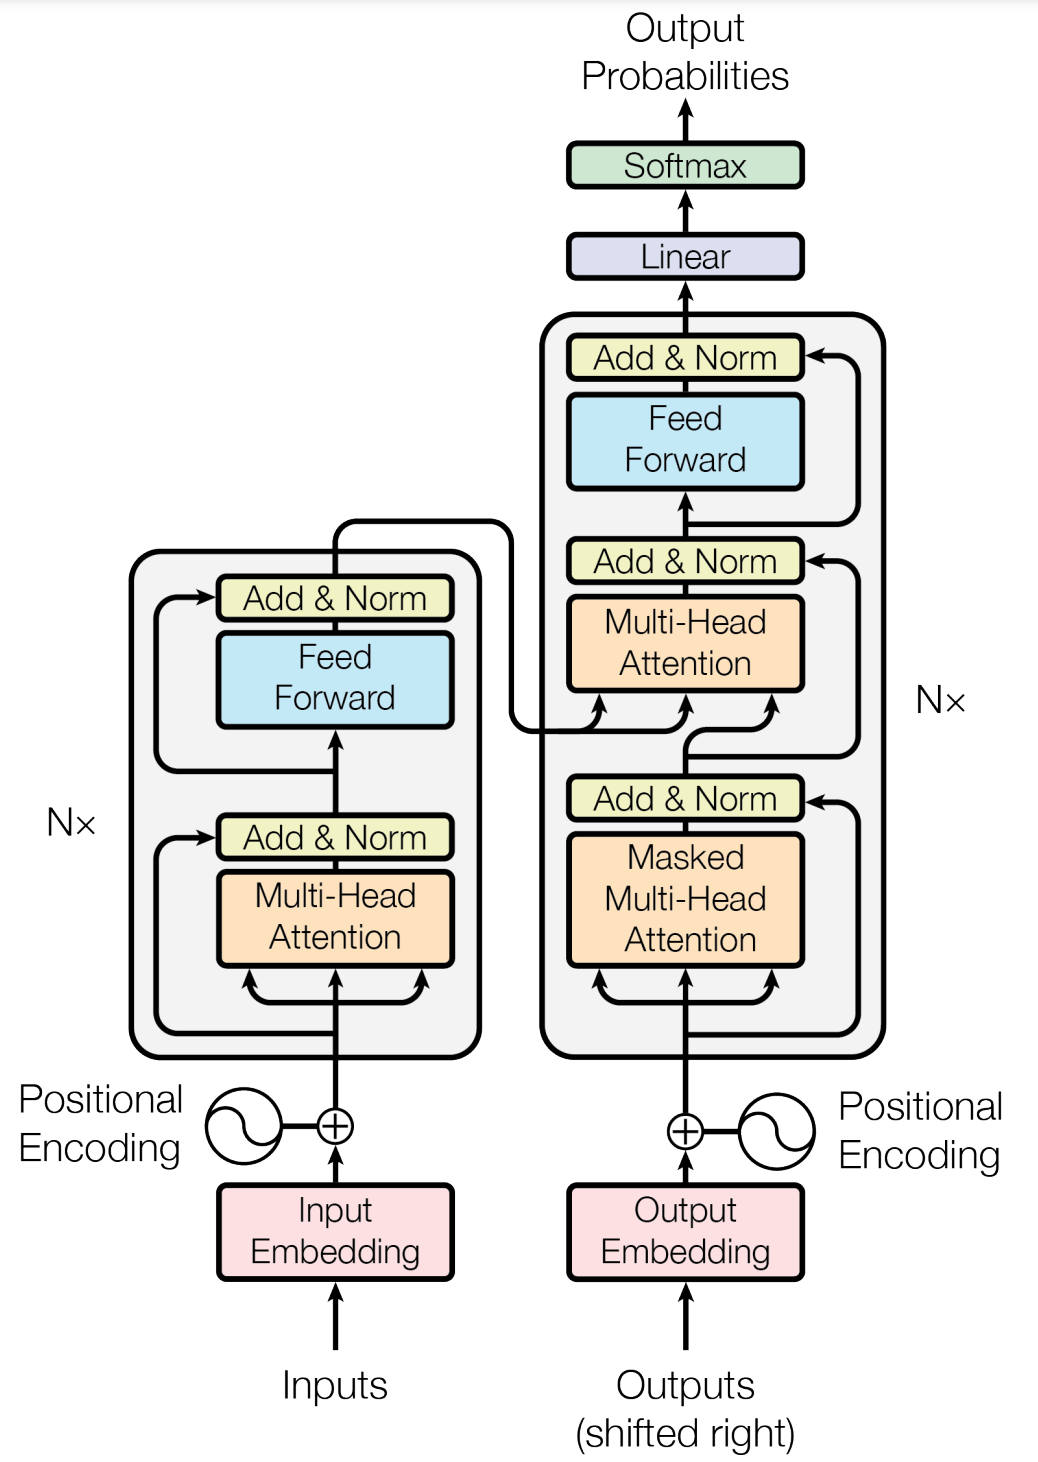
\includegraphics[scale=0.1]{Transformer_architecture}
    \centering    
\end{figure}

\subsection{Architecture}

Tokenizer

Positional encoding


Transformer layer (encoder/decoder)


Unidirectional / bi-directional




\section{Variational Autoencoder}


- Encoder network which parameterizes the approximate posterior distribution $q(z|x$) of latent variables $z$ given the data $x$.
- Prior $p(z)$
- Decoder with distribution $p(x|z)$. 
- Note that we get the joint distribution $p(z)p(x|z) = p(x,z)$

ELBO and why

ELBO is a lower bound for the log likelihood of the data.

Maximizing ELBO w.r.t $\phi, \theta$  will concurrently (simultaneously)
- Approximately maximize the marginal likelihood $p_\theta(x)$ 
	- Generative model gets better
- Minimize the KL-divergence of the approximate posterior to true posterior. 
	- $q(z|x)$ becomes better

\subsection{VQVAE}

with and without decorr

\subsubsection{Codebook}


\section{Self-supervised Learning}
Self-supervised learning (SSL) has had great success in natural language processsing and computer vision in recent years. 

Establish context:
What is supervised learning? 
What is unsupervised learing?
How does SSL differ from the previous two?

Explain why we care:
What are som of the promises of SSL, how and why can it be usefull?
Its relationship to representation learning?

Explain where we are now:
What are the different flavours of SSL? Contrastive vs non-contrastive
What are some of the issues? Collapse, where encodes produce uniformative or constant vectors.
Some mainstream models? 
Where has it seen success?\\\\

Joint embedding architecture: An architecure where two networks are trained to produce similar embeddings for different views of the same data. A popular joint embedding architecture is the siamese network architecture \cite{siamese}, in which the two networks share the same weights. In models with such architecture, the existence of trivial solutions, such as both networks ignoring input and produce identical constant embeddings, is a major issue. This issue is reffered to as \textit{collapse} of the model.

Augmentations for creating different views. The role of augmentations, types etc. 


Autoassociative SSL - Autoencoder type - Essentialy try to make composition the identity despite a compression. 

Contrastive SSL includes both positive and negative samples. The loss function of contrasitive SSL attempts to minimize the distance of positive sample pairs (+,+) and (-,-), and maximize the distance between negative sample pairs (+,-) and (-,+).\\\\

vs non contrastive


\subsection{Barlow Twins}
What is it?

How does it work?

\subsection{VIbCReg}
What is it?

VIbCReg \cite{lee2024vibcreg} is a non-contrastive SSL model based on VICReg \cite{bardes2022vicreg}. It has a joint embedding architecture,

How does it work?


\section{MaskGIT}

The Masked Generative Image Transformer is a generative transformer model for image synthesis developed by Google Research. The novelty of the model lies in the token generation. Unlike popular autoregressive generative transformers, who treat images as a sequence of tokens, MaskGIT introduces an image synthesis paradigm using a bi-directional transformer decoder. This means that during training MaskGIT learns to predict tokens in all directions, an intuitively more natural way to consider images. At inference time MaskGIT starts out with a blank canvas and predicts the entire image, and iteratively keeps and conditions on the most confident pixels.\\\\

\TODO{Intuitive introduction of masked modelling. Figures and such.}

The model assumes a tokenization procedure for stage 1, and in the original paper they used VQGAN \cite{VQGAN}. As MaskGIT only focuses on improving stage 2, present only that part. 

\subsection{Prior learning}

Start out with a sequence $s$ (b,n) of codebook indeces corresponding to a discrete latent representation $z_q$. Determine the proportion of tokens to mask according to the mask scheduling function $\gamma(t)\in (0,1]$. 
Sample a random subset of $s$ and replace values by [MASK] token in order to create the masked sequence $s_M$ (b,n). By a forward pass of the bi-directional transformer with $s_M$ as input obtain unnormalized logits (b,n,K), defining a distribution over the codebook indeces at each element. Calculate the loss as the binary cross-entropy of the logits and $s$. 

\subsection{Iterative decoding}

The bi-directional transformer could in principle predict all [MASK] tokens and generate a sample in a single pass by simply sampling from the logits obtained from a forward pass of an all masked sequence. However, there are challenges with this approach. In their original article \todo{spør om siteringsstil, og fiks denne setningen} \cite{chang2022maskgit} proposes a novel non-autoregressive decoding method to sythesize samples in a constant number of steps.\\\\

The decoding process goes from $t = 0$ to $T$. To genereate a sample at inference time one starts out with a all masked sequence which we denote by $s_M^{(0)}$. At iteration $t$ the model predicts the probabilities for all the [MASK] tokens, $p(\hat{s}_{ij}^{(t)}|s_M^{(t)})$, in parallell. Then at each masked entry $ij$ we sample a token index based on its predicted distribution.  

\subsection{Masking design}
\TODO{Could it be interesting to investigate different masking designs for time series? Is cosine the ubiquitous choice}



\end{document}